\documentclass[uplatex,b5j,11pt]{jsbook}
\title{周期}

\usepackage[dvipdfmx]{graphicx}
\usepackage{fancybox}
\usepackage{amsmath,amssymb}
\usepackage{multicol}
\usepackage{ascmac}
\usepackage{booktabs}
\usepackage[dvipdfmx]{graphicx}
\usepackage[dvipdfmx]{color}
\usepackage{makeidx}
\usepackage{colortbl}
\usepackage{amsthm}
\usepackage{my-default}
\usepackage{tikz}
\usepackage{tikz-cd}


\begin{document}
\chapter{Introduction}
周期とは適当な関数を適切な範囲で積分したものである.
適当なの意味はものによって変わりうる.
ここではContesvich-Zagier予想や数論で出てくる周期に関する話ができればと思う.
自分の興味としては
\begin{itemize}
\item 計算との関連.
\begin{itemize}
  \item 計算可能実数や実閉体のモデル理論との関連.
  \item 数論的な対象が計算可能とは,どういう意味か?
\end{itemize}
\item 数論幾何的な対象の深い理解
\begin{itemize}
\item ドラムの定理との関連
\item モチーフ,数論的基本群との関連
\end{itemize}
\end{itemize}
このノートは周期について自分が話したことを中心にまとめ直すものとする.


%\chapter{リーマン面の理論}
\section{周期積分、ヤコビ多様体}
実際にリーマン面の理論の後半を読み,周期の関連を見る.

\subsection{位相幾何からの準備}
議論をする上で最低限のホモトピー論,ホモロジー論を定義する.
\begin{screen}
\begin{dfn}
 $X$上の2つの連続なpath $f,g: [0,1] \to X$に対し,連続写像$H:[0,1] \times [0,1] \to X$で
 $H(0, \cdot) = f(\cdot), H(1, \cdot)$となるものが存在するす時,$f,g$は\textbf{ホモトピック}という.
\end{dfn}
\end{screen}

\begin{screen}
\begin{dfn}
 $X$と$x \in X$に対して基点,つまり始点と終点が$x$となる連続なpath全体を$F$と表す.$\alpha, \beta \in F$に対して,
 \begin{equation*}
 \alpha \cdot \beta (t) = \begin{cases}
    \alpha(2t) & ( t \le 1/2) \\
    \beta(2t-1) & (t \ge 1/2)
  \end{cases}
 \end{equation*}
とすると,これは積構造を定める.
これをホモトピーによる同値関係で割ったものを\textbf{基本群}といい$\pi(X,x)$で表す.
すぐ計算すればわかるように,基本群上でも上で定めた積構造がwell-definedであり,この演算について群になる.
また,弧状連結である等,基点のとり方によらない場合は$\pi(X)$と表すこともある.
\end{dfn}
\end{screen}

\begin{screen}
\begin{dfn}
 $A \subset X$に対し,$F(x, 0) = x , F(x, 1) \in A , F(a, 1) = a$となる写像$F$を変位レトラクトという.
これは,$X$上の恒等写像と$A$へのレトラクション($A$への制限が恒等写像になるもの)の間のホモトピーの存在を意味する.
この時,$id$とレトラクトはホモトピー同値になる.ただし$A$に写像が制限されていないので,ホモトピー同値はホモトピックと同値になる.
\end{dfn}
\end{screen}

ホモロジー・コホモロジーについて定義する.
具体的な話を書きすぎると死んでしまうが,

\begin{itemize}
\item 特異ホモロジー
\item 単体ホモロジー
\item 特異コホモロジー
\item Kronecker積
\end{itemize}
について説明する.

$\Delta^n := \{ x \in \mathbb{R}^{n+1} \mid  \sum x_i =1, \forall x_i \ge 0 \}$とする.
$S_n(X) := \{f: \Delta^n \to X \mid f \mbox{は連続写像}\}$とし,
$C_n(X) := \oplus_{f \in S_n(X)} \mathbb{Z}$とする.
$i_j: \Delta_n \to \Delta_{n+1}$を第$j$成分を0にし,それ以降は一つずらしとする写像とする.
$d: S_n(X) \to S_{n-1}(X), \sum_{j} f \mapsto (-1)^j f \circ i_j$とする.
すると$d_n \circ d_{n+1} = 0$となり,

\begin{screen}
\begin{dfn}
$\mathcal{U} =  \{U_i\}_{i \in I}$を$X$の開被覆とする. 任意の有限個の$i_1, \ldots ,i_k \in I$に対し$ \cap U_i$が可縮な時,$\mathcal{U}$を\textbf{単純被覆}という.
$X$が$n$次元多様体であって,
\end{dfn}
\end{screen}

\subsection{ポアンカレの補題とドラムの定理}

% \chapter{第一回周期セミナー@12/01}
12月1日に行われた周期セミナーの初回で説明である.
第一回では層の定義と層のコホモロジーについて議論した.

周期の数論的な関係を見るために,代数的なDeRhamの定理を\url{https://arxiv.org/pdf/1302.5834.pdf}に基づきまとめる.

ここでは層と層係数のコホモロジーを使ってドラムの定理を計算する.
そこで最初に層の準備、及びスペクトル系列についての内容を記載する.

\begin{itemize}
  \item 微分形式のなす層を定義し,それがfineであることを示す.
  \item パラコンパクト位相空間上のfine sheafはacyclic
  \item 二重複体のコホモロジーからacyclic resolutionの時のコホモロジーの同型を示す.
  \item コホモロジーの同型とPoincareの補題から可微分多様体と複素多様体の場合のドラムの定理を示す.
  \item GAGAと複素多様体の時のドラムの定理から射影代数多様体の場合にドラムの定理を示す.
  \item チェックコホモロジーを使って代数多様体のドラムの定理を広い範囲に拡張している.
\end{itemize}

コホモロジーのNotaiton
\begin{itemize}
  \item $\mathcal{H}^k(A())$: 層のcomplexのk次のImage/Ker
  \item $\mathfrak{h}^k(T(L))$: 層のcomplex$L$をアーベル群の完全関手で飛ばした先のコホモロジー.
  \item $H^K(U,L)$: 層$L$のcomplexの$U$でのセクションのコホモロジー.
  \item $\mathbb{H}^k(X, L)$: 二重複体(今回は$L$のGodement resolution)に対するTotalのコホモロジー
\end{itemize}
余力があればやりたいこと
\begin{itemize}
  \item $M$の特異コホモロジーと定数層のコホモロジーの(大域切断)一致
\end{itemize}

\begin{thm}
\begin{equation*}
H^n(X,\Omega_{alg}) = H^n(X_{an},\mathbb{C})
\end{equation*}
\end{thm}
\section{層の議論}
ここでは層と層の間の射について定義する.
\begin{itemize}
\item 層の層化側の定義
\item 層の貼り合わせの条件
\item 環つき空間の射
\item $f:(X, O_X) \to (Y, O_Y)$から作れる層.
\end{itemize}


\subsection{層の定義}

\begin{screen}
\begin{dfn}
 任意の開集合$U \subset X$に対し,$\mathcal{F}(U)$が対応し,
 $v \subset U$なら制限写像$|_V: \mathcal{F}(U) \to \mathcal{F}(V)$が存在し、以下を満たす時
 $\mathcal{F}$を前層という.
 \begin{itemize}
   \item $F(\emptyset) = 0$
   \item $|_U:F(U) \to F(U) = id$
   \item $|_W \circ |_V = |_W$
 \end{itemize}
 前層$\mathcal{F}$が任意の開集合$U$とその開被覆$\{U_i\}$に対し,以下を満たす時層という.
 \begin{itemize}
   \item $s \in F(U)$に対し,$s|_{U_i}=0$の時,$s=0$.
   \item $s_i \in F(U_i)$に対し,$s_i|_{U_{ij}}= s_j|_{U_{ij}}$となる時,$s \in U$で$s|_{U_i} = s_i$となる.
 \end{itemize}
\end{dfn}
\end{screen}


\begin{epl}
位相空間$\mathbb{C}$を考え,その開集合$U$に対し,
\begin{equation*}
F(U) := \{f:U \to \mathbb{C} \mid f \mbox{is continuous} \}
\end{equation*}
とする.$|_U$を定義域の制限で定める.この時$F$は層になる.
\end{epl}

\begin{lem}
前層$\mathcal{F}$が層であることは
任意の開集合$U$とその開被覆$\mathcal{U}$に対し,
\begin{equation*}
 0 \to \mathcal{F}(U) \to \prod_{U_{\alpha} \in \mathcal{U}} \mathcal{F}(U_{\alpha})
   \to \prod F(U_{\alpha} \cup U_{\beta})
\end{equation*}
がexact.
\end{lem}
\begin{proof}
自明.ちゃんと証明を書く場合はまた今度.
単射性は左側の完全性
張り合わせは右側の全射性に対応
\end{proof}

前層$\mathcal{F}$に対し,
\begin{equation*}
    \mathcal{F}_x := \varinjlim_{x \in U}\mathcal{F}(U)
\end{equation*}
これを前層の茎(stalk)という.

前層の層化を定義する
\begin{screen}
\begin{dfn}[層化]
$X$上の前層$\mathcal{F}$に対し,
\begin{equation*}
\mathcal{G}(V)= \{ (s_x) \in \coprod_{x \in V} \mathcal{G}_x \mid \forall x, \exists U_x ,f  \in \mathcal{F}(U_x) \mbox{s.t. } \forall y \in U_x, s_y = f_y \}
\end{equation*}
で定めた層$\mathcal{G}$を層化という.
\end{dfn}
\end{screen}


\begin{lem}
上で定めた$\mathcal{G}$は層になる.
\end{lem}
\begin{proof}
単射性を示す.
開被覆$\{\mathcal{U_i}\}$に対し,$s|_{U_i} = 0$なら
$s = (s_x)$とした時にすべての$s_x$に対し$0$となるので$s = 0$となる.
張り合わせは$s_i|_j = s_j|_i$の時,$s = (s_x)$を$x \in U_i$に対しては$s_x =s_i|_x$とする.
この時,$x \in U_{ij}$に対し,$s_i|_x = s_j|_x$となるので,$s$はwell-definedであり,$s|_{U_i} = s_i$となる.
\end{proof}

\begin{lem}
自然な射$f: \mathcal{F} \to \mathcal{G}$とすると,$\forall x \in X$に対し,
$\mathcal{F}_x \simeq \mathcal{G}_x$を誘導する.
\end{lem}


\begin{screen}
\begin{dfn}
$X$のOpen Base $\mathcal{B}$に対して層の性質を満たすものを,$\mathcal{B}$-sheafという.
\end{dfn}
\end{screen}

\begin{lem}
$\mathcal{B}$-shaef $\mathcal{F}$に対し,$X$上の層$\mathcal{G}$で$\forall U \in \mathcal{B}$に対し,$\mathcal{F}(U) = \mathcal{G}(U)$となるものが存在する.
\end{lem}
層化同様の方法で
\begin{equation*}
\mathcal{G}(V)= \{ (s_x) \in \prod \mathcal{G}_x \mid \forall x, \exists U_x ,f  \in \mathcal{F}(U_x) \mbox{s.t. } \forall y \in U_x, s_y = f_y \}
\end{equation*}
とすればこれは層になる.
$\mathcal{F}(U) = \mathcal{G}(U)$はinductive limitのuniversalityからもわかるし,
層化の構成で作ったものとの同型を層の性質からも直接示せる.
$\mathcal{F}(U) \\mathcal{G}(U)$は$\{U_x \}$を取ることにより,開被覆となり,全射性がわかる.また単射性も層の性質からわかる.

層の定義を満たす具体例を紹介する.
層の典型的な例は位相空間$X$に対し,$F(U)$を$U$から$\mathbb{R}$への連続関数全体です.


\begin{rem}
 上を用いるとある開被覆$\{U_i\}$と$U_i$上の層$\mathcal{F}_i$が存在し,$\mathcal{F}_i|_j = \mathcal{F}_j|_i$ならば
 $X$上の層$\mathcal{F}$で$F|_i = \mathcal{F}_i$となるものが存在する
 ($\{U_i\}$とその開部分集合はopen baseになるので)
 なので,スキーム同士を張り合わせる場合は上の条件を満たせば問題ない.
\end{rem}

\subsection{層の射}
$X$上の層の射の定義と射の全単射を定義する
\begin{screen}
\begin{dfn}
$f: \mathcal{F} \to \mathcal{G}$とは

\begin{tikzcd}
  \mathcal{F}(U) \ar[r, "f_U"] \arrow[d, "|_V"'] & \mathcal{G}(U) \ar[d, "|_V"] \\
  \mathcal{F}(V) \ar[r, "f_V"] & \mathcal{G}(V)
\end{tikzcd}

が可換となること
\end{dfn}
\end{screen}

開被覆で定まる層があれば,それをもとに全体に張り合わせられる.

\begin{screen}
\begin{dfn}
$X$上の層$f: \mathcal{F} \to \mathcal{G}$に対し,$\mathrm{Ker}f$を
\begin{equation*}
    U \to \mathrm{Ker} (f(U))
\end{equation*}
で定める層とし,$\mathrm{Im}f$を
\begin{equation*}
    U \to \mathrm{Im} (f(U))
\end{equation*}
の層化で定義する.

\end{dfn}
\end{screen}

\subsection{層の射が誘導する層}
位相空間の間の連続写像が誘導する層
$f: X \to Y$に対し
$X$上の層$\mathcal{F}$に対し,

層の延長

\subsection{環つき空間と射}

環つき空間

環つき空間の間の射
\begin{screen}
\begin{dfn}
環$R$に対し,素イデアル全体のなす集合$\mathrm{Spec}R$に$D(f)$を開基とする位相をいれる.
\end{dfn}
\end{screen}

スキームや代数多様体が環つき空間になっていること(これはRemark)



\input{date/20191201/cohomologyofsheaf}
% 


\chapter{1/05発表}
前回の準備をもとに代数的なドラムの定理を実際に証明する
今回の話す内容は以下の通りである.
\begin{itemize}
    \item 前回の復習(定義と最低限の性質のみ)
    \item スペクトル系列の定義と性質
    \item 二重複体からスペクトル系列の作成方法
    \item スペクトル系列を用いた実、複素の場合のドラムの定理の証明
    \item 代数的なドラムの定理の証明.ただし、SerreのGAGAを前提にする.
    \item ドラムの定理の一般の代数多様体への拡張
    \item GAGAへの理解の向上.
\end{itemize}

\section{前回の復習}
前回は層の定義と層係数コホモロジーの計算方法や性質を説明した.
\begin{itemize}
  \item Godement Resolutionの定義
  \item Godement Resolutionのセクションを取る操作は完全関手である.
  \item Flabby Sheafの定義
  \item $\mathbb{R}$上の微分加群の層がFine Sheafであり、特にacyclic
\end{itemize}


\section{Spectral Sequence and double complex}
\begin{dfn}
$(E, F^pE, E^{p,q}_r, d_r^{p,q}:E_r^{p,q} \to E_r^{p+r, q-r+1})$がスペクトル系列とは
\begin{itemize}
  \item $F^pE$はfiniteなFiltration.すなわち,十分小さい$p^0$以下の全ての$p$に対し,$F^pE =E$,十分大きい$p_1$以上の全ての$p$に対し,$F^pE=0$.
  \item $d \circ d = 0$
  \item $\forall (p,q) \in \mathbb{Z}^2$,$\exists r_0 \in \mathbb{Z}_{\ge 1}$で$r \ge r_0$に対し,$d_r^{p,q} = d_r^{p-r, q+r-1} = 0$となる.
  \item $\mathrm{Ker}d_r^{p,q}/ \mathrm{Im}d_r^{p-r,q+r-1} \simeq E_{r+1}^{p,q}$
  \item $E^{p,q}_{\infty} = F^pE^{p+q}/F^{p+1}E^{p+q}$
ただし,$E_{\infty}^{p,q}$は十分大きい$r$に対しては$E_r^{p,q}$が一致し、それを表す.
\end{itemize}
\end{dfn}

特殊なスペクトル系列の場合の性質について示す.
- $E_{\infty}^{p,q}$が単純な場合のlimit
- $E_r$ termが単純な場合のlimit

必要な範囲の証明に留める.

今回は二重複体からスペクトル系列を構成するのが目標である.

二重複体には$n$に対し,$a+b=n$となるものの中で$K^{a,b}\neq 0$となる$(a,b)$が有限という条件を課す.
これに対して$E_1^{p,q}:= H^q(K^{p,q})$,$E^{p+q}:=H^{p+q},(Tot(K^{p+q}))$となるスペクトル系列を構成する.

二重複体からスペクトル系列を構成する手順を説明する.

前提となる道具の定義
\begin{itemize}
  \item 次数1の有限二重次数完全対
  \item 導来対
\end{itemize}
メインの定理: 二重次数完全対からスペクトル系列が構築できる.
応用:
\begin{itemize}
  \item フィルター付けされた複体から次数1の有限二重次数完全対の構築
  \item 二重複体のToTからフィルター付けししたスペクトル系列の構築
\end{itemize}

\begin{dfn}
アーベル群$D,E$に対し,$i:D \to D,j:D \to E, k:E \to D$が与えられとする.
$(D,E,i,j,k)$が以下を満たす時 \textbf{完全対}という.
\begin{itemize}
  \item $\mathrm{Ker}j = \mathrm{Im}i$
  \item $\mathrm{Ker}k = \mathrm{Im}j$
  \item $\mathrm{Ker}i = \mathrm{Im}k$
\end{itemize}
\end{dfn}

\begin{dfn}
完全対$(D,E,i,j,k)$に対し,以下の操作で作った対を導来対という.
\begin{itemize}
    \item $D':=\mathrm{Im}i$
    \item $E':=\mathrm{Ker}(j \circ k)/ \mathrm{Im}(j \circ k)$
    \item $i'=i|_{D'}$
    \item $j'(a):= \overline{j(b)}(i(b)=a)$
    \item $k'(a + \mathrm{Im}(j \circ k )):= k(a)$
\end{itemize}
\end{dfn}

\begin{prop}
上の構成がwell-definedであり,完全対となる.
\end{prop}
\begin{proof}
$E',j',k'$についてwell-defined性を示す.
\begin{itemize}
    \item $E'$: 
$\mathrm{Ker}k = \mathrm{Im}j $より, $j \circ k\circ j \circ k = 0$となるので,$E'$はwell-defined.
\item $j'$:
$j(b) \in \mathrm{Ker}k$より$j(b) \in \mathrm{Ker}(j \circ k)$となる.
さらに,$i(b)=i(b')=a$とすると,$b-b' \in \mathrm{Ker}i = \mathrm{Im} k$となり,$j(b-b') \in \mathrm{Im}(j \circ k)$となるので,well-defined.
\item $k'$: $b \in \mathrm{Im}(j \circ k)$とすると,$K \circ j = 0$より言える.
\end{itemize}
完全性を示す.とり方から
$j'\circ i' = 0, k' \circ j' =0, i' \circ k' = 0$はすぐわかる.
$Im i' \subset Ker j'$

\end{proof}


$r$次導来対は上の構成を$r$回繰り返したものとして定義する.

\begin{dfn}
二重次数つき完全対とは
\end{dfn}

実際に層係数コホモロジーについて同型を示す

\section{The Hypercohomology of a complex of sheaves}
$X$上の層のcomplex $\mathcal{L}^{\bullet}$に対し,そのGodment Resolutionのなす二重複体を以下で定義する.
\begin{equation*}
K := \bigoplus_{p,q} K^{p,q} = \bigoplus_{p,q} \Gamma(X, C^p \mathcal{L}^q).
\end{equation*}
$\mathbb{H}(X, \mathcal{L})$をTotal Coplexの定めるCohomologyとする.

今あり得るコホモロジーは
様々な複体があるので,それらに対する表記を定める
層の二重複体を
\begin{itemize}
    \item 層の複体が作る, コホモロジーの層$\mathcal{H}^p(\mathcal{L}^{\bullet})$
    \item 層の大域切断が作る群の$p$次コホモロジー$H^p(X,L^n)$
    \item 層のTotal Complexが作る群のコホモロジー$\mathbb{H}^p(X,L):= H(\oplus_{a+b=p} C^{a}L^{b})$
    \item 層の複体の大域切断が誘導する群の複体から作るコホモロジー$h^p(\Gamma(X, \mathcal{L})$
\end{itemize}
これをいくつかの条件下でどういう関係にあるかを示す.


Total Cohomologyは層のコホモロジーの拡張と捉えられる.

$\mathcal{L}$に対し,$0 \to \mathcal{L} \to 0$という複体を考えると,
$\mathbb{H}(X, \mathcal{L}):= h^k(\Gamma(X, C^{\bullet} F))$となる.

目的はDeRhamの定理
実の場合は微分加群の層はFineなのでAcyclicになる.

ここで言いたいこと
\begin{itemize}
  \item Godement Resolutionの場合のコホモロジーの関係
  \item 層の複体の間のQuasi isoを与えた場合にGlobal Sectionのコホモロジーがどうなるか?
  \item Acyclicな層のcpxの場合のTotal Cohomologyどうなるか?
  \item DeRhamの定理への応用
\end{itemize}


今この場合に二重複体の作るスペクトル系列$E^{p,q}_1, E^{p,q}_2, E^{n}, F^pE_n$について確認する.
まず
$K^{p,q}:=\Gamma(X, C^p \mathcal{L}^q)$となる.
$E^{p,q}_1:= H^k(X, \mathcal{L}^{\bullet})$


$\mathbb{C}$上の代数多様体(局所的には$\mathbb{C}[X_1,\dots,X_n]/(f_1, \ldots, f_m))$の作るAffine Schemeと同型)とした時,
そこから,複素解析的な空間を作れる
$X^a= \{ x \in \mathbb{C}^n \mid f_j(x) = 0 \}$
$O^{X^{a}}$を$X^a$上の正則関数全体が作る層を$(f_1,, \ldots, f_m)$で割った層とする.

$\mathbb{C}$上の代数多様体$X$から複素解析的な空間$X^a$を作る操作は関手的であり,これは連接層についても拡張できる.
($X$上の連接層に対して,$X^{an}$の連接層を対応させられる)

また射としては$\phi: X^{a} \to X$が取れるので、層同士の間にも射が誘導される.
$\phi^* \mathcal{F} \sim \mathcal{F}^a$となり,
$H^i(X, \mathcal{F}) \to H^i(X_h, \phi^* \mathcal{F})$が誘導される.
これは$X$がsmooth projectiveの場合,同型になる.

$\mathcal{F}$が代数的な微分形式の層だとすると,$\mathcal{F}^a$は解析的な微分形式の層になる.

よって,
代数的な微分形式のなす層の複体のGGodement Resolutionが作るGlobal Sectionの二重複体に対する,
$E_1^{p,q}$は$H^P(X, \Omega_{alg}^q)$
解析的な方は
$E_1^{p,q}$は$H^P(X^a, \Omega_{an}^q)$となり,GAGAにより一致する.
(本当はスペクトル系列が誘導する射の同型も必要だが)よって,コホモロジーが一致する.
$$
H^{*}\left(X_{\mathrm{an}}, \mathbb{\mathbb { C }}\right) \simeq
\mathbb{H}^{*}\left(X_{\mathrm{an}}, \mathbb{C}^{\bullet}\right) \simeq
\mathbb{H}^{*}\left(X_{\mathrm{an}}, \Omega_{\mathrm{an}}^{\bullet}\right) \simeq
\mathbb{H}^{*} \left(X, \Omega_{\mathrm{alg}}^{\bullet}\right)
$$
よって言えた.
% 
\chapter{20200322}
今回話したいこと
\begin{itemize}
    \item モチベーション
    \item 層の定義とB-sheafの定義.
    \item 環つき空間と$O_X$-modの層
    \item アフィンスキームの層(イメージ)
    \item $M$加群から準連接層の構成
    \item 準連接層の定義と性質
    \item アフィンスキーム上の準連接層と加群の誘導する層の関係
    \item 連接層の定義と性質
    \item アフィンスキームの場合の準連接層のコホモロジー
    \item 射影スキームの構成
    \item 射影スキームによるtwist
    \item 射影スキーム上の準連接層,連接層の特徴づけ
    \item 射影スキーム上の連接層のコホモロジーの計算
\end{itemize}

\subsection{モチベーション}
このセミナーではしばらく周期の話をする。
\begin{itemize}
\item $X$: $\overline{\mathbb{Q}}$上の代数多様体
\item $Z \subset X$: closed subvariety
\item $\gamma \in H_n(X^{an}, Z^{an}, \mathbb{Z})$:相対特異ホモロジー類
\item $\omega \in H_{dR}^n(X, \mathbb{Z})$をde Rhamコホモロジー類
\end{itemize}
この時$[X, Z, n ,\gamma, \omega]$を抽象的周期という.
前回のセミナーにて代数的なドラムの定理を示した。
改めて定理を記述すると
$X$を$\mathbb{C}$上の射影代数多様体とした時,
\begin{equation*}
  H^q(X_an, \mathbb{C}) = \mathcal{H}^q(X, \Omega_{alg})
\end{equation*}
となる.

前回はこれを二重複体の理論を使って証明した.
ただし,解析と代数との直接の関係はSerreのGAGAを用いて使った.
そこで今回次回の二回はSerreのGAGAを目標とする.
GAGAは射影代数多様の連接層とその複素化が作る連接層に対応があることを示すが。
連接層の一般論自体はそれ以前の論文で行われている。
またGAGA自体がスキーム論以前なので、スキーム論的にまとめ直したい.

ということで今回は準連接層や連接層を構成し,特に射影スキーム上の連接層のコホモロジーを計算したい。

\subsection{Preliiminary}

\subsection{global sectionで生成される層と準連接層}

\begin{screen}
\begin{dfn}
  
\end{dfn}
\end{screen}


大域切断で生成される層
準連接層の定義
$A$加群$M$が作る層
準連接層の操作に対する性質
アフィンスキーム上の準連接層の性質
連接層の定義と性質
ネーター環上のアフィンスキームの場合の連接層と加群の関係
Principal Open setを使ったチェックコホモロジーの計算
射影スキームの定義と基本的な性質
射影空間の性質
射影スキーム上の準連接層と連接層の構成
射影スキームの場合の次数つき加群と連接層の関係
(Remarkするだけ上野 定理5.21)
射影空間の連接層のコホモロジーの計算

\section{Coherent sheaves on scheme}
\subsection{sheaves of modules}

\begin{screen}
\begin{dfn}
 $(X, O_X)$をringed spaceとする.$X$上のアーベル群の層$\mathcal{F}$が$O_X$-加群であるとは,
 \begin{itemize}
   \item $X$の任意のopen set $U$に対し,$F(U)$は$O_X(U)$加群となる.
   \item $V \subset U$に対し,以下となる.

   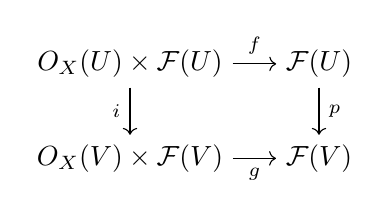
\begin{tikzpicture}[auto]
   \node (a) at (0, 1.2) {$O_X(U) \times \mathcal{F}(U)$};
   \node (x) at (2.4, 1.2) {$\mathcal{F}(U)$};
   \node (b) at (0, 0) {$O_X(V) \times \mathcal{F}(V)$};
   \node (y) at (2.4, 0) {$\mathcal{F}(V)$};
   \draw[->] (a) to node {$\scriptstyle f$} (x);
   \draw[->] (x) to node {$\scriptstyle p$} (y);
   \draw[->] (a) to node[swap] {$\scriptstyle i$} (b);
   \draw[->] (b) to node[swap] {$\scriptstyle g$} (y);
   \end{tikzpicture}
\end{itemize}
\end{dfn}
\end{screen}


この時,$\mathcal{F},\mathcal{G}$のテンソル積,$\mathcal{F} \otimes_{O_X} \mathcal{G}$を
\begin{equation*}
U \mapsto \mathcal{F}(U) \otimes_{O_X(U)} \mathcal{G}(U)
\end{equation*}
の層化したものを$\mathcal{F} \otimes_{O_X} \mathcal{G}$で表す.
また$(\mathcal{F} \otimes_{O_X} \mathcal{G})_x = \mathcal{F}_x \otimes_{O_X, x} \mathcal{G}_x$となる.
これは\ref{tensor module}で示す.


\begin{screen}
\begin{dfn}
$(X, O_X)$加群$\mathcal{F}$に対し,$\mathcal{F}$が$x \in X$でglobal sectionで生成されるとは,
\begin{equation*}
  O_{X,x} \otimes \mathcal{F}(X) \twoheadrightarrow \mathcal{F}_x
\end{equation*}
となること.
$\forall x \in X$でglobal sectionで生成される時,$\mathcal{F}$はglobal sectionで生成されるという.
$S \subset \mathcal{F}(X)$に対し,$\{s_x \mid s \in S\}$が$\mathcal{F}_x$を生成する時$S$で生成されるという.
\end{dfn}
\end{screen}

\begin{lem}
 $\mathcal{F}$がglobal sectionで生成されていることと$O_X^{(I)} \twoheadrightarrow \mathcal{F}$と同値.
\end{lem}
\begin{proof}
$O_X^{(I)} \twoheadrightarrow \mathcal{F}$ならば$\mathcal{F}$がglobal sectionで生成されていることを示す.

   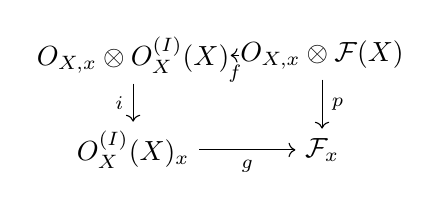
\begin{tikzpicture}[auto]
   \node (a) at (0, 1.2) {$O_{X,x} \otimes O_X^{(I)}(X) $};
   \node (x) at (2.4, 1.2) {$O_{X,x} \otimes \mathcal{F}(X)$};
   \node (b) at (0, 0) {$O_X^{(I)}(X)_x$};
   \node (y) at (2.4, 0) {$\mathcal{F}_x $};
   \draw[->] (a) to node {$\scriptstyle f$} (x);
   \draw[->] (x) to node {$\scriptstyle p$} (y);
   \draw[->] (a) to node[swap] {$\scriptstyle i$} (b);
   \draw[->] (b) to node[swap] {$\scriptstyle g$} (y);
   \end{tikzpicture}

が成り立ち,$i$は$O_X^{(I)}$は$O_X$加群としてglobal sectionで生成されているので全射.
また,$g$は仮定から全射となる.よって$p$は全射となるので,global sectionで生成されている.

逆を示す.$S$として$\mathcal{F}(X)$を取ることにより,必ず$\mathcal{F}$を生成する$S$が存在する.
また,$e_s \in O_X^S(U)$を$e_s(s) = 1, e_s(t) = 0$となる元とし,
$O_X^{S}(U) \to \mathcal{F}(U), \sum_{s \in S} a_s e_s \mapsto a_s s_U$とすれば,
これは層の間の射となり,全射性も言える.
\end{proof}


\begin{screen}
\begin{dfn}
$(X, O_X)$加群の層$\mathcal{F}$が\textbf{quasi coherent shaef}とは$\forall x \in X$に対し,$x \in U$が存在し,
\begin{equation*}
  O_X^{(J)}|_U \to O_X^{(I)}|_U \to \mathcal{F}|_U
\end{equation*}
がexactとなることを言う.
\end{dfn}
\end{screen}

\subsection{Quasi-Coherent Sheaves on an affine scheme}
$X = \mathrm{Spec}A$の時にquasi-coherent sheafを構成する.
$M$を$A$-modする.
$\tilde{M}$という$O_x$-加群を構成する.
\begin{equation*}
\tilde{M}(D(f)) := M_f = M \otimes_A A_f
\end{equation*}
とする.
$D(g) \subset D(f)$の時,$V(g) \supset V(f)$なので,
$\cup_{f \in p}p  = \sqrt{(f)} \ni g$となる.よって$g^n = fb$とかける.これより

\begin{alignat*}{2}
 A_f & \to &  \ A_g \\
 \frac{a}{f^m} & \mapsto & \ \frac{b^ma}{g^{mn}}
\end{alignat*}

が定まり,それの誘導する射

\begin{alignat*}{2}
 M_f & \to &  \ M_g \\
 \frac{x}{f^m} & \mapsto & \ \frac{b^m x}{g^{mn}}
\end{alignat*}

が定義される.
この時$\{D(f)\}$上で$\tilde{M}$が$\mathcal{B}$-sheafになることを示す.
\begin{align*}
  & X = \cup D(f_i) \\
\Leftrightarrow & X = D \left(\sum (f_i) \right) \\
\Leftrightarrow & V \left(\sum (f_i) \right) = \emptyset
\end{align*}
この時,$\sum f_i = (1)$より,$\sum a_i f_i = 1$とかける.
よって$a_i$が$0$でない$f_i$を使い,$X = \cup_{i=1}^n D(f_i)$とかける.

$X$のfinite open coveringについて,$X$について層の定義を満たすことを示せば十分である.
$X$についての条件を満たせれば,$X=D(f)$の時について示せる,それは$D(f) \cup D(f_i)$がAffineになるので,$D(f)$というスキームのfinte open coveringについて示せる.
また,finite open coverの時に言えれば,compactなのでopen coverに対し,affin finte open coverが取れ、そこ上で成り立つことを示せばよい。
特に
\subsection{Coherent sheaves}


\begin{lem}
\label{tensor module}
$X$上の$O_X$加群$\mathcal{F},\mathcal{G}$のテンソル積,$\mathcal{F} \otimes_{O_X} \mathcal{G}$を
$\mathcal{F} \otimes_{O_X} \mathcal{G}(U) := \mathcal{F}(U) \otimes_{O_X(U)} \mathcal{G}(U)$とすると層になる
また$(\mathcal{F} \otimes_{O_X} \mathcal{G})_x = \mathcal{F}_x \otimes_{O_X, x} \mathcal{G}_x$となる.
\end{lem}
環つき空間をスキームの場合に限定して示す. 局所的なので、$X$をアフィンスキームと思って良い.

\begin{lem}
$S^{-1}N \otimes M \sim S^{-1}(N \otimes M)$
\end{lem}
真面目に元をおえば示せる.


\begin{lem}
$S^{-1}(N \otimes M) \sim S^{-1}N \otimes_{S^{-1}R} S^{-1}M$
\end{lem}
これは$S^{-1}N = N \otimes S^{-1}R$より
\begin{equation*}
  S^{-1}N \otimes_{S^{-1}R} S^{-1}M \sim N \otimes S^{-1}R \otimes_{S^{-1}R} S^{-1}M \sim N \otimes S^{-1}M \sim  S^{-1}(N \otimes M)
\end{equation*}
となる.

これを使うことにより,スキームに対しては成り立つことがわかる.
おそらく,一般の場合は上と近い形で
$O(V) \otimes_{O(U)} M(U) \otimes N(V) \to M(V) \otimes N(V)$と
$N(U) \otimes M(U) \to O(V) \otimes N(U) \otimes M(V)$とを使いながら,これのらindcutive limitが一致することを示せばよいはず。


\section{Projective Scheme}

Projcetive Schemeの定義をする.
GAGAの対象となる射影代数多様体は$\mathbb{P}^n_{\mathbb{C}}$のclosed subschemeである.

\begin{dfn}
$B$が次数つき$A$代数であるとは
$B = \oplus B_n$とかけ,$B_n B_m \subset B_{n+m}$となること
\end{dfn}



\begin{lem}
  $f \in B_+$をdegree $r$のhomogeneousな元とする.
\begin{enumerate}
  \item canonicalな射は$\theta: D_+(f) \to \mathrm{Spec}B_{(f)}$同相となる
  \item $D_+(g) \subset D_+(f)$の時,$\alpha = g^r f^{- \mathrm{deg} g}$とする.
  この時$\theta(D_+(g)) = D(\alpha)$
  \item 自然な射$B_{(f)} \to B_{(g)}$は$(B_{(f)})_{\alpha} = B_{(g)}$をinduceする.
  \item その他いろいろ
\end{enumerate}
\end{lem}
1を示す.
方針は以下の通り.
\begin{itemize}
  \item $\mathrm{Proj}B$が$\mathrm{Spec}B$の部分位相であることを示す.
  \item 環の間の射を用いて自然な射を誘導し,連続であることを示す
  \item 射が全射であることを示す
  \item 射が単射であることを示す.
  \item 開写像であることを示す.
\end{itemize}

\begin{screen}
\begin{dfn}
  $X_i:=\mathrm{Spec}A[T_iT_j^{-1}]$とすると$X_{ij} = X_{ji}$となるので,これを張り合わせたものを$A$のProjective Spaceといい$\mathbb{P^n}_A$で表す.
  Projective Spaceのclosed subschemeをProjective Schemeという.
\end{dfn}
\end{screen}

% \section{層の議論}
ここでは層と層の間の射について定義する.
\begin{itemize}
\item 層の層化側の定義
\item 層の貼り合わせの条件
\item 環つき空間の射
\item $f:(X, O_X) \to (Y, O_Y)$から作れる層.
\end{itemize}


\subsection{層の定義}

\begin{screen}
\begin{dfn}
 任意の開集合$U \subset X$に対し,$\mathcal{F}(U)$が対応し,
 $v \subset U$なら制限写像$|_V: \mathcal{F}(U) \to \mathcal{F}(V)$が存在し、以下を満たす時
 $\mathcal{F}$を前層という.
 \begin{itemize}
   \item $F(\emptyset) = 0$
   \item $|_U:F(U) \to F(U) = id$
   \item $|_W \circ |_V = |_W$
 \end{itemize}
 前層$\mathcal{F}$が任意の開集合$U$とその開被覆$\{U_i\}$に対し,以下を満たす時層という.
 \begin{itemize}
   \item $s \in F(U)$に対し,$s|_{U_i}=0$の時,$s=0$.
   \item $s_i \in F(U_i)$に対し,$s_i|_{U_{ij}}= s_j|_{U_{ij}}$となる時,$s \in U$で$s|_{U_i} = s_i$となる.
 \end{itemize}
\end{dfn}
\end{screen}


\begin{epl}
位相空間$\mathbb{C}$を考え,その開集合$U$に対し,
\begin{equation*}
F(U) := \{f:U \to \mathbb{C} \mid f \mbox{is continuous} \}
\end{equation*}
とする.$|_U$を定義域の制限で定める.この時$F$は層になる.
\end{epl}

\begin{lem}
前層$\mathcal{F}$が層であることは
任意の開集合$U$とその開被覆$\mathcal{U}$に対し,
\begin{equation*}
 0 \to \mathcal{F}(U) \to \prod_{U_{\alpha} \in \mathcal{U}} \mathcal{F}(U_{\alpha})
   \to \prod F(U_{\alpha} \cup U_{\beta})
\end{equation*}
がexact.
\end{lem}
\begin{proof}
自明.ちゃんと証明を書く場合はまた今度.
単射性は左側の完全性
張り合わせは右側の全射性に対応
\end{proof}

前層$\mathcal{F}$に対し,
\begin{equation*}
    \mathcal{F}_x := \varinjlim_{x \in U}\mathcal{F}(U)
\end{equation*}
これを前層の茎(stalk)という.

前層の層化を定義する
\begin{screen}
\begin{dfn}[層化]
$X$上の前層$\mathcal{F}$に対し,
\begin{equation*}
\mathcal{G}(V)= \{ (s_x) \in \coprod_{x \in V} \mathcal{G}_x \mid \forall x, \exists U_x ,f  \in \mathcal{F}(U_x) \mbox{s.t. } \forall y \in U_x, s_y = f_y \}
\end{equation*}
で定めた層$\mathcal{G}$を層化という.
\end{dfn}
\end{screen}


\begin{lem}
上で定めた$\mathcal{G}$は層になる.
\end{lem}
\begin{proof}
単射性を示す.
開被覆$\{\mathcal{U_i}\}$に対し,$s|_{U_i} = 0$なら
$s = (s_x)$とした時にすべての$s_x$に対し$0$となるので$s = 0$となる.
張り合わせは$s_i|_j = s_j|_i$の時,$s = (s_x)$を$x \in U_i$に対しては$s_x =s_i|_x$とする.
この時,$x \in U_{ij}$に対し,$s_i|_x = s_j|_x$となるので,$s$はwell-definedであり,$s|_{U_i} = s_i$となる.
\end{proof}

\begin{lem}
自然な射$f: \mathcal{F} \to \mathcal{G}$とすると,$\forall x \in X$に対し,
$\mathcal{F}_x \simeq \mathcal{G}_x$を誘導する.
\end{lem}


\begin{screen}
\begin{dfn}
$X$のOpen Base $\mathcal{B}$に対して層の性質を満たすものを,$\mathcal{B}$-sheafという.
\end{dfn}
\end{screen}

\begin{lem}
$\mathcal{B}$-shaef $\mathcal{F}$に対し,$X$上の層$\mathcal{G}$で$\forall U \in \mathcal{B}$に対し,$\mathcal{F}(U) = \mathcal{G}(U)$となるものが存在する.
\end{lem}
層化同様の方法で
\begin{equation*}
\mathcal{G}(V)= \{ (s_x) \in \prod \mathcal{G}_x \mid \forall x, \exists U_x ,f  \in \mathcal{F}(U_x) \mbox{s.t. } \forall y \in U_x, s_y = f_y \}
\end{equation*}
とすればこれは層になる.
$\mathcal{F}(U) = \mathcal{G}(U)$はinductive limitのuniversalityからもわかるし,
層化の構成で作ったものとの同型を層の性質からも直接示せる.
$\mathcal{F}(U) \\mathcal{G}(U)$は$\{U_x \}$を取ることにより,開被覆となり,全射性がわかる.また単射性も層の性質からわかる.

層の定義を満たす具体例を紹介する.
層の典型的な例は位相空間$X$に対し,$F(U)$を$U$から$\mathbb{R}$への連続関数全体です.


\begin{rem}
 上を用いるとある開被覆$\{U_i\}$と$U_i$上の層$\mathcal{F}_i$が存在し,$\mathcal{F}_i|_j = \mathcal{F}_j|_i$ならば
 $X$上の層$\mathcal{F}$で$F|_i = \mathcal{F}_i$となるものが存在する
 ($\{U_i\}$とその開部分集合はopen baseになるので)
 なので,スキーム同士を張り合わせる場合は上の条件を満たせば問題ない.
\end{rem}

\subsection{層の射}
$X$上の層の射の定義と射の全単射を定義する
\begin{screen}
\begin{dfn}
$f: \mathcal{F} \to \mathcal{G}$とは

\begin{tikzcd}
  \mathcal{F}(U) \ar[r, "f_U"] \arrow[d, "|_V"'] & \mathcal{G}(U) \ar[d, "|_V"] \\
  \mathcal{F}(V) \ar[r, "f_V"] & \mathcal{G}(V)
\end{tikzcd}

が可換となること
\end{dfn}
\end{screen}

開被覆で定まる層があれば,それをもとに全体に張り合わせられる.

\begin{screen}
\begin{dfn}
$X$上の層$f: \mathcal{F} \to \mathcal{G}$に対し,$\mathrm{Ker}f$を
\begin{equation*}
    U \to \mathrm{Ker} (f(U))
\end{equation*}
で定める層とし,$\mathrm{Im}f$を
\begin{equation*}
    U \to \mathrm{Im} (f(U))
\end{equation*}
の層化で定義する.

\end{dfn}
\end{screen}

\subsection{層の射が誘導する層}
位相空間の間の連続写像が誘導する層
$f: X \to Y$に対し
$X$上の層$\mathcal{F}$に対し,

層の延長

\subsection{環つき空間と射}

環つき空間

環つき空間の間の射
\begin{screen}
\begin{dfn}
環$R$に対し,素イデアル全体のなす集合$\mathrm{Spec}R$に$D(f)$を開基とする位相をいれる.
\end{dfn}
\end{screen}

スキームや代数多様体が環つき空間になっていること(これはRemark)



\chapter{GAGA}
GAGAでは射影代数多様上の層とそのanalyticなものが定めるコホモロジーの一致や圏同値を示す.
ここでは,最初にanalytic spaceとその上の層を定義する.
その後代数多様体に対し,代数多様体のanalytic化を定義し,射影代数多様体の場合の関係について示す.
\section{preliminary}
GAGAでは既知とされることを一定まとめておく.
ここでは層と環のflatについて説明する.
\subsection{sheaf}
GAGAでは層を普段とは異なる方法で定義しているため、その点に言及しておく.
GAGAやFACでは層を以下で定義している.
\begin{screen}
\begin{dfn}
\begin{itemize}
以下の組を層という.
  \item 位相空間$X$
  \item $x \in X$に対し,アーベル群$\mathcal{F}_x$が対応する.
  \item $\mathcal{F}$を集合としては$\mathcal{F}_x$のdisjoin unionとなる位相空間
\end{itemize}
$\pi: \mathcal{F} \to X$を$f \in \mathcal{F}_x$の時$\pi(f)=x$とする.
さらに
\begin{itemize}
  \item 任意の$f \in \mathcal{F}$に対し,$f \in \mathcal{F}$の近傍$V$と$\pi(f)=x$の近傍$W$で$V,W$が同相となるものが存在する.
  \item $f,g$に対し, $-f , f + g$がcontinuos(加法は$\pi(f) = \pi(g))$の時のみ.
\end{itemize}
\end{dfn}
\end{screen}

この時,$\Gamma(\mathcal{F}, U) := \{ s \in  \Hom_{conti}(U,\mathcal{F}) \mid \pi \circ s = id_u, \}$とすると,
これはアーベル群となる.
また,通常よくある層の公理を満たす.sectionなので明らかにわかる.非自明なのは連続性だけだが、貼り合わせを考えることでわかる.

逆にこちらの層を定義とする.
\begin{prop}
層の定義は互いに同値である.
\end{prop}
最初に$X, \mathcal{F}_x, \mathcal{F}, \pi$を定める.
$X$は元の位相空間のままとし,$\mathcal{F}_x := \varinjlim \mathcal{F}(U)$とする.$\mathcal{F}$は$\mathcal{F}_x$のdisjoint unionで定める.
$\mathcal{F}$の位相を定める.
$t \in \mathcal{F}(U)$と$x \in U$に対し,$\phi_x^U: \mathcal{F}(U) \to \mathcal{F}_x$とする.
$[t, U]$を$\{\phi_x^{U}(t)\}$のなす集合とする.
$\mathcal{F}$の$[t, U]$の生成する位相とする.実際にこの位相が局所同相性や演算の連続性を満たすことを示す.
実際$\phi_x^U(t)$の近傍として$[t,U]$がとれ,これは$U$と同相になる.
また,$f \mapsto -f$は$[t, U]$の逆像が,$[-t, U]$を対応させるのでのでcontinousであり,
$(f, g) \mapsto f + g$での$[t, U]$の逆像は
$\cup_{x \in U, f_x \in \mathcal{F}_x}(f_x+\phi_x^U(t), -f_x)$となり,さらに以下となる.
\begin{equation*}
\cup_{x \in U, f_x \in \mathcal{F}_x}(f_x+\phi_x^U(t), -f_x) = \cup_{x \in U, f_x \in \mathcal{F}_x} [g_x + \phi_x^U(t), V_{f_x} \cup U] \times [-g_x, V_{f_x} \cup U]
\end{equation*}
ただし$g_x \in \mathcal{F}(V_{f_x} \cup U)$で$\phi_x^{V_{f_x} \cup U}(g_x) = f_x$である.
$x$の表記がかぶっているのは微妙.
これはOpenなので連続である.

\subsection{direct imageとinverse image}
層にはdirect imageとinverse imageと呼ばれる操作がある。

\begin{screen}
\begin{dfn}
$f: X \to Y$と$X$上の層$\mathcal{F}$と$Y$上の層$\mathcal{G}$が存在する時に,\textbf{direct image}$f^*\mathcal{F}$を
$Y$の開集合$U$に対し,
\begin{equation*}
f^* \mathcal{F}(U) = F(f^{-1}(U))
\end{equation*}
で定める.
また,\textbf{inverse image}$f^{-1}\mathcal{G}$を$X$の開集合$V$に対し,
\begin{equation*}
f^{-1} \mathcal{G}(V) = \varinjlim_{f(V) \subset U} \mathcal{G}(U)
\end{equation*}
で定める.特に,$f^{-1}\mathcal{G}_x = \mathcal{G}_{f(x)}$となる.
\end{dfn}
\end{screen}

direct imageを使い層をextensionする.
\begin{screen}
\begin{dfn}
$V$を$X$の閉集合とする.$i : V \to X$に対し,
$V$上のsheaf$\mathcal{F}$に対し,direct image $i^*\mathcal{F}$を層の\textbf{extension}という.

この時
\begin{equation*}
    i^* \mathcal{F}(U) = \mathcal{F}(U \cap V)
\end{equation*}
となり,stalkは
\begin{equation*}
    i^*\mathcal{F}_x = \begin{cases}
        \mathcal{F}_x & x \in Y \\
        0 & otherwise
    \end{cases}
\end{equation*}
となる.
\end{dfn}
\end{screen}

\begin{rem}
  $V$が閉集合出ない場合は,$\mathcal{F}_x = 0$と限らない.
\end{rem}

\subsection{Flat couple}
flatとcompletionについて議論する.

\begin{screen}
\begin{dfn}
$R$-加群$M$が\textbf{flat}とは
\begin{equation*}
 0 \to M_1 \to M_2 \to M_2 \to 0
\end{equation*}
がexactの時
\begin{equation*}
 0 \to M_1 \otimes M \to M_2 \otimes M\to M_2 \otimes M \to 0
\end{equation*}
がexactとなること.テンソル積は右完全なので$M_1 \otimes M \to M_2 \otimes M$が単射であることと同値.
\end{dfn}
\end{screen}

これは$Tor$を使って議論することができる.
Torは
$N$のProjective Resolutionを取る.つまり射影加群$P_n$とすると,
\begin{equation*}
P_{n+1} \to P_n \to \ldtos \to P_1 \to N \to 0
\end{equation*}
がexactの時,
\begin{equation*}
P_{n+1} \otimes M \to P_n \otimes M  \to \ldtos \to P_1 \otimes M \to N \otimes M \to 0
\end{equation*}
とする.
この時
\begin{equation*}
\mathrm{Tor}_i(N, M) = \mathrm{Ker}(P_n \otimes M \to P_{n-1} \otimes M) / \mathrm{Im}(P_{n+1} \otimes M  \to P_n \otiesm M)
\end{equation*}
で定義する.

\subsection{Algebraic Variety}
GAGAで出てくる代数多様体について解説する.

$X$を位相空間とする.
\begin{equation}
\mbox{閉集合による降下列は停留する.} \tag{A}
\end{equation}
これは閉集合のなす集合が極小元を持つことを指す.


\begin{prop}
  \begin{itemize}
    \item $X$が条件Aを満たす時,$X$はcompact
    \item $X$が条件$A$を満たす時,subspaceも条件$A$を満たす.
    \item $X$が条件$A$を満たす$Y_i$のfinite unionでかける時,$X$は条件$A$を満たす.
  \end{itemize}
\end{prop}
\begin{proof}
  $X$の閉集合のなす集合で$\cap F_i = \emptyset$となったとする.$I$を適当な順序数と同一視し,
  $F_0, F_0 \cap F_i, \ldots \cap_{i=1}^n F_i$とすると,これは停留するので,有限個の集合で空となる.よってcompact
次に,停留しないとすると$A$を含む閉集合で停留しないものが取れるので、矛盾.
finite unionなので、それぞれについてのなす閉集合をunionしても閉となり,言える.
\end{proof}

$X$がirreducibleとは$X = F_1 \cup F_2$の時,$X = F_1$か$X=F_2$となること.

\subsection{Locally closed subsets of an affine space}

$x_0 \in K^n$に対し,$O_x= \{P(x)/Q(x) \mid Q(x_0) \neq 0\}$とする.
$\mathscr{J}_{x}(V)$を$x \in V$の時は$V$上で0になる関数,$x \notin V$の時は
$\mathscr{J}_{x}(V)=\mathscr{O}_{x}$とする.

この時,$\mathcal{J}(V)$はcoherent sheafになる.

\subsection{Definition of the structure of an algebraic variety}

以下を$K$上の代数多様体という.
\begin{itemize}
    \item $X$は位相空間
    \item $O_x$は$X$上の$K$に値を取る関数のgermのなす層$\mathcal{F}(X)$のsubsheaf
\end{itemize}
さらに
$X$のfinite open coveringで,$V_i$はaffine spaceのlocally closed subspace $U_i$とisomorphicとなる.
それと
$X \times X$の対角成分は閉という仮定をおく.

つまり, sepaterdかつneotherな$K$上のスキームを考える.


\section{Analytic Spaces}
最初にローカルな世界でanalyticを定義する.
\begin{screen}
\begin{dfn}
$U \subset \mathbb{C}^n$が\textbf{analytic}とは$\forall x \in U$に対し,ある$x$の近傍$W \subset \mathbb{C}^n$上の正則関数$f_1, \ldots ,f_k$が存在し,
\begin{equation*}
  U \cap W = \{x \in W \mid f_1(x) = \ldots  f_k(x) = 0 \}
\end{equation*}
となること.
\end{dfn}
\end{screen}

これは複素多様体とは限らないが,
$U \cap W$上で$\frac{\partial f_i}{\partial x_j}$のrankが$U$のとり方によらない時,$\mathbb{C}^n$の閉部分多様体そのものであり,特に複素多様体になる.

\begin{lem}
$U \cap W$上で$\frac{\partial f_i}{\partial x_j}$のrankが$U$のとり方によらない時,$U$は複素多様体である.
\end{lem}
\begin{proof}
多様体の局所座標系を$U_i,\phi_i = (z_1,\ldots, z_n)$とする.
この時,rankが$k$なので$z,f$ともに順序を適切に入れ替えて$\frac{\partial f_j}{z_i}_{i,j \le k}$のrankが$k$となるようにする.
$F: U \to \mathbb{C}^n$を$F(x) = (f_1(x), \ldots, f_k(x), z_{k+1},\ldots, z_{n})$とすると,これは$\phi_i^{-1}(U) \to \mathbb{C}^n$に拡張され$\phi(x)$上で逆関数定理からその近傍で微分同相であることがわかる.
よって,$(f, z)$による局所座標をいれられる.また,
$U \cap W$は$(z_{k+1}, \ldots, z_n)$と微分同相であることがわかるので,複素多様体になる.
\end{proof}

$U$の位相を調べると.$U$はlocally closedとなり,またlocally compactとなる.($\mathbb{C}^n$の開集合も閉集合はlocally compactなのでその共通部分も同様)
\begin{screen}
\begin{dfn}
位相空間$X$の部分集合$A$がlocally closedとは,以下の同値な条件を満たすことである.
\begin{enumerate}
  \item あるopen set $U$と closed set $V$が存在し,$A = U \cap V$となること.
  \item $x \in A$に対し,ある$x$の近傍$W$が存在し,$A \cap W$が$W$上closedであること
\end{enumerate}
\end{dfn}
\end{screen}
\begin{lem}
上が同値である.
\end{lem}
\begin{proof}
1. $\Rightarrow$ 2. は$W$として$U$を取れば良い.この時$A \cap U = V \cap U$となるので,$U$上closed. \\
2. $\Rightarrow$ 1.を示す.これは$A$の閉包上$A$が開集合であることを示せばよい.そうすれば,
$A = \overline{A} \cap U$となる.$W$が開集合の時だけ示せばよい.
この時,$A \cap W =  \overline{A} \cap W$となる.
それは$\overline{A} \subset \overline{A \cap V} \cup \overline{A \cap (X \setminus V)}$
であり,$\overline{A} \cap V \subset \overline{A \cap V} \cap V$となる.
さらに$\overline{A} \cap V \subset \overline{A \cap V} \cup V = A \cap V$より
$\overline{A} \cap V = A \cap V$となる.これより$A \cap V$は$\overline{A}$上開集合となる.
$A = \cup_{x \in A} A \cap V$より$A$は$\overline{A}$上開集合となる.
\end{proof}

ここからは$U$上の層を定義する.
$X$上$\mathbb{C}$への連続関数が作る層を$\mathcal{C}(X)$とする.
$\mathcal{C}(\mathbb{C}^n)$を$\mathbb{C}$に値を取る連続関数のなす層とし,$\mathcal{H}$を$C^n$上の正則関数のなす層とする.


$U \subset \mathbb{C}^n$上の正則関数のなす層を$\mathbb{C}^n$の連続関数のなす層から$U$上の連続関数のなす層への写像を使い定義する.

$\forall x \in U$に対し,$\epsilon_x:\mathcal{C}(\mathbb{C}^n)_x \to \mathcal{C}(U)_x$が定義される.
この写像での$\mathcal{H}_x$の像を$\mathcal{H}_{x,U}$とする.
$\epsilon_x: \mathcal{H}_x \to \mathcal{H}_{x, U}$のkernelを$\mathcal{A}_x(U)$と表す.これは$U$上ゼロになった正則関数全体となる.
今後しばしば$\mathcal{H}_{x, U}= \mathcal{H}_{x}/ \mathcal{A}_x(U)$で定める.
$\mathcal{A}(U), \mathcal{H}_{U}$は$U$上の層となる.
%つまり$\epsilon: \mathcal{C}(\mathbb{C}^n) \to \mathcal{C}(U)$による定義域のsub sheaf $\mathcal{H}$のImageで層$\mathcal{H}_U$を定める.

この定義では$U$が多様体でなくても定義できる.この$(U,H_U)$を\textbf{analytic space}という.
またanalytic spaceの間の射を以下で定義する.
\begin{screen}
\begin{dfn}
 $U,V$をanalytic spaceとする.$\phi: U \to V$が\textbf{holomoprhic}とは以下を満たすことである.
 \begin{itemize}
   \item $\phi$は連続
   \item $\mathcal{H}_{\phi(x), V} \to \mathcal{H}_{x, U}, f \mapsto f \circ \phi$がwell-definedであること.
         つまり$f \circ \phi \in \mathcal{H}_{x, U}$となること.
 \end{itemize}
\end{dfn}
\end{screen}

analytic subsetやholomorphicは直積で保たれる.
つまり$U, V$がanalyticなら$U \times V$はanalyticで$\phi, \phi'$がholomorphic$\phi \times \phi' : U \times U' \to V \times V'$はholomorphic.

\subsection{The notion of an analytic space}
先程はAffineな場合のanalytic spaceを定義したのでここからは一般の位相空間の場合のanalytic spaceを定義する.

\begin{screen}
\begin{dfn}
 位相空間$X$と$\mathcal{C}(X)$の部分層$\mathcal{H}_X$が\textbf{analytic space}であるとは,以下を満たすことである.
 \begin{itemize}
   \item $X$の開被覆$\{V_i\}$が存在し,$V_i$はあるaffine analytic space$U_i$と同相であり,
   また,ここから$\mathcal{H}_X|_{V_i}$と$\mathcal{H}_{U_i}$が層として同型である.
   \item $X$はハウスドルフ
 \end{itemize}
\end{dfn}
\end{screen}
$X$の開部分集合:$V$がchartとはあるアフィンanalytic space$U$とanaltyic isomorphismが存在すること.

\subsection{Analytinc Sheaves}
Analytic Spaceの構造層$\mathcal{H}_X$は環の層なので,$H_X$加群をAnaltyic shaefという.

$Y$を$X$のclosed analytic subspaceとする.
この時,$\mathcal{A}_x(Y) \subset \mathcal{H}_{x, X}$を$f$の$Y$での制限がzeroとなるものとする.
特に$x \notin Y$の時は$\mathcal{A}_x(Y) = \mathcal{H}_x(Y)$とする.この時$\mathcal{A}_x(Y)$の元は$f$は$\mathcal{H}_x(Y)$の元をかけても$x \in Y$の近傍で$0$のままなので,$\mathcal{A}_x(Y)$の元となる.特に$\mathcal{A}(Y)$は$\mathcal{H}_X$加群となる.

\begin{prop}
  \begin{itemize}
    \item $\mathcal{H}_X$はCoherent sheaf of rings.
    \item $Y$が$X$のclosed analytic subspace of $X$の時,$\mathcal{A}(Y)$をcoherent analytic sheafとなる.
  \end{itemize}
\end{prop}
\url{http://www-fourier.ujf-grenoble.fr/~demailly/analytic_geometry_2019/sheaves_and_analytic_sets.pdf}
この辺を見る

\subsection{A neighborhood of a point in an analytic space.}

\section{The analytic space associated to an algebraci variety}
最初に$\mathbb{C}$上のalgebraic varietyとregular mapを定義する.

\begin{screen}
\begin{dfn}
有限生成$\mathbb{C}$代数$R$に対し,$(\mathrm{Spm}R, R)$を\textbf{アフィン代数多様体}といい、
2つのアフィン代数多様体$(\mathrm{Spm}R, R)$と$(\mathrm{Spm}S, S)$に対して$\mathbb{C}$準同型写像$\psi: S \to R$と$\psi$から定まる写像$\psi^a: \mathrm{Spm}R \to \mathrm{Spm}S$が存在する時,
$(\psi, \psi^a)$を(正則な)射という.
\end{dfn}
\end{screen}
$I$を含む極大イデアル全体の集合を$V(I)$とすると,$V(I)$全体を閉集合とする位相が定まり,Zariski位相という.

\begin{rem}
  スキームと同様に$f \in R$に対し,$D_m(f):= R_f$とする層が定まりこれにより代数多様体も局所環つき空間として考えられる.
\end{rem}

\subsection{Definition of the analytic space associated to an algebraic variety.}

これに付随するanalytic spaceが定義できる.
代数多様体はlocalにはAffine代数多様体であり,その時$\mathrm{Spm}R$は$\mathbb{C}^n$のZariski閉集合に対応する.
よってこれらにはanalytic spaceの構造が定まり,実は全体ではりあわせることができる.

アフィン代数多様体の場合に$\phi: V \subset \mathbb{C}^n \to W \subset \mathbb{C}^m$が\textbf{regular}とは
$\phi = (\Phi_1, \ldots, \Phi_m)$で各$\Phi_i$が多項式でかけること.

\begin{prop}
There exists on $X$ a unique structure of an analytic space such
 that, for every chart $\phi : V \to U$, the Z-open set $V$ is open, and $\phi$ is an analytic
 isomorphism of V (equipped with the analytic structure induced by that of $X$)
 onto $U$ (equipped with the analytic structure defined in $n^o 1$).
\end{prop}

\subsection{Relations between the local ring at a point and the ring of holomorphic functions at that point}
$X$をalgebraic varietyとする.$x \in X$に対し,$O_x$,$\mathcal{H}_x$が定まる.
上の補題からregular functionaはholomorphic functionなので,$\theta: O_x \to \mathcal{H}_x$が定まり,
$x$上で0になるものは0になるままなので,$\theta(m_x) \subset m_{\mathcal{H}_x}$となり,$\hat{\theta}: \hat{O_x} \to \hat{\mathcal{H}}_x$が定まる.

以下2つの命題は同時に示す.
証明が全く読めない...
\begin{prop}
 $\hat{\theta}: \hat{O}_x \to \hat{\mathcal{H}}_x$はbijective
\end{prop}

\begin{prop}
 $\mathcal{A}_x(Y)$ is generated by $\theta(\mathscr{J}_x(Y))$
\end{prop}

\begin{proof}
まず$X = \mathbb{C}^n$の時に示す.この時は$\hat{O}_x = \mathbb{C}[[x_1,\dots,x_n]] = \hat{\mathcal{H}}_x$となるので,成り立つ.
\end{proof}
\subsection{Relations between the usual topology and the Zariski topology of an algebraic variety.}

\subsection{An analytic criterion for regularity}

\begin{prop}
 $T,X$が代数多様体で$p: T \to X$がregular bijectiveであり,$p$がanalytic isomならbiregular isomである.
\end{prop}

\section{Thre correspondence between algebraic sheaves and coherent analytic sheaves}

\subsection{The analytic sheaf associated to an albgeraic sheaf}
$X$を$\mathbb{C}$上のalgberaic varietyとする.
それに対し,$X^h$を$X$に付随するanalytic spaceとする.
$\mathcal{F}'$を$X \to X_h$に対するinverse imageとする.

$\mathcal{F}^h:= \mathcal{F}' \otimes \mathcal{H}$とする.

\begin{prop}
 \begin{itemize}
     \item Functor $\mathcal{F}^h$はexact functor
     \item algebraic sheaf $\mathcal{F}$に対し,$\alpha: \mathcal{F}' \to \mathcal{F}^h$はinjective
     \item $\mathcal{F}$がcoherent algebraic sheafなら $\mathcal{F}^h$もcoherent analytic sheafになる.
 \end{itemize}
\end{prop}



$O_x$加群の層ををalgebraic sheafといい,$M$をanalytic spaceとした時,$O_{M}$加群の層をanalytic sheafという.


\section{Projective varieties. Statements of the theorems.}
GAGAのmain theoremについて説明する

$X$をprojective variety,ここでは$\mathbb{P}^r(\mathbb{C})$の閉部分多様体する.

\begin{thm}
$X$上のcoherent algeberaic sheaf $\mathcal{F}$に対し,
\begin{equation*}
 \epsilon: H^q(X, \mathcal{F}) \to H^q(X^h, \mathcal{F}^h)
\end{equation*}
はisomorphism
\end{thm}

\begin{thm}
$\mathcal{F}, \mathcal{G}$を$X$上のcoherent algebraic shaefとする.この時,
\begin{equation*}
 \mathrm{Hom}(\mathcal{F}, \mathcal{G}) \sim \mathrm{Hom}(\mathcal{F}^h, \mathcal{G}^h)
\end{equation*}
\end{thm}

\begin{thm}
$X^h$上のcoherent analytic sheaf $\mathcal{M}$に対し,$X$上のalgberaic sheaf $\mathcal{F}$で$\mathcal{F}^h = \mathcal{M}$となるものが存在する
\end{thm}

これを一つずつ示す.
\section{Proof of theorem 1}
証明の前にいくつか補題を示す.

\begin{lem}
$X$上の層$\mathcal{F}$に対し,$X \subset Y$のとき,
$Y$のopn set $U$に対し,$\mathcal{F}^e(U)$を
\begin{equation*}
  U \mapsto \begin{cases}
    \mathcal{F}(U) & (if U \subset X) \\
    0 & (otherwise)
\end{cases}
\end{equation*}
で定める前層の層化とする.
この時,
\begin{equation*}
\mathcal{F}^e_x =
\begin{cases}
    \mathcal{F}_x & (if x \in X) \\
    0 & (otherwise)
\end{cases}
\end{equation*}
となる.
\end{lem}
\begin{proof}
前層のとり方から明らか.
\end{proof}

\begin{lem}
この時,cohomologyは一致する.
つまり,$X \subset Y$の時
\begin{equation*}
 H^q(X, \mathcal{F}) = H^q(Y, \mathcal{F}^e)
\end{equation*}
となる.
\end{lem}
\begin{proof}
check cohomologyで考えるとよい.
$Y$の任意のopen coverに対し,
Fineな十分小さいOpen Cover$\mathcal{U} = \{U_i\}$を取ると
$U_i \subset X$以外では$\mathcal{F}(U_i) = 0$としてよい.
よって十分細かいopen coverに対し,
$H(\{U_i \cap X\}, \mathcal{F}) = H(\mathcal{U}, Y)$となる.
これより,inductive limitwをとっても一致する.
\end{proof}

$X$でのコホモロジーと射影空間のコホモロジーが一致するので,射影空間で考える.

射影空間の場合にコホモロジーが一致することを示す.

基本的な方針は以下の通り.

\begin{enumerate}
  \item $O$の場合のanalyticなコホモロジーを計算
  \item $O(m)$の場合の代数的なコホモロジーを計算
  \item $O(m)$の場合にインダクションを使って示す.
  \item 連接層の場合にインダクションを使って示す.
\end{enumerate}

\paragraph{$O$の場合のanalyticなコホモロジーを計算.}
$H^q(X^h, O^h)$は$q=0$の場合は$X^h$上正則な関数全体であり,$X$はコンパクトなので$\mathbb{C}$になる.
$q>0$の時,0になる.ドルボーの定理から$H^{0,q}(X^h, O^h)$と一致するがこれが消える理由はよくわからない.

\paragraph{$O(m)$の場合の代数的なコホモロジーを計算}
射影空間の代数的なコホモロジーは以下となる.

\begin{thm}
$R$をネーター環,$S=\mathbb{P}_R^n$とする.
  \begin{enumerate}
    \item $S \simeq \oplus_{n \in \mathbb{Z}}H^0(X, O_X(m))$
    \item $0 < i < n$に対し,$H^i(X, O_X(m)) = 0$
    \item $H^n(X, O_X(-n-1)) \simeq R$
    \item $H^0(X, O_x(m)) \times H^n(X, O_X(-m-n-1)) \to H^n(X, O_X(-n-1))$はperfect pairing
  \end{enumerate}
\end{thm}

\begin{proof}
\paragraph{$S \simeq \oplus_{n \in \mathbb{Z}}$}
自明.$H^0(X, O_X(m)) = S_m$で$m < 0$の時,$S_m =0$からわかる.
\paragraph{$H^n(X, O_X(-n-1)) \simeq R$}
$C^{n-1}(\mathcal{U}, O_X(m)) \to C^n(\mathcal{U}, O_X(m))$を構成する.
$U_j:= D_+(x_j)$とし,$U_{j_0\ldots j_k} = \cap_{i=1}^k U_{j_i}$とする.
$\mathcal{U}:= \{U_j \mid j=0, \ldots, n\}$
$\Gamma(U_{j_0 \ldots j_p}, O_x(m)) = \{\frac{f}{(x_0\ldots x_n)^{\ell}} \mid \mathrm{deg}f = \ell(p+1) +m\}$となる.
$ \delta: C^{n-1}(\mathcal{U}, O_x(m)) \to C^n(\mathcal{U}, O_xm)$を構成する.
具体的に書くと以下となる.
\begin{align*}
  \oplus_{i=0}^m S(m)_{(x_0 \ldots \hat{x_i} \ldots x_n)} & \to S(m)_{(x_0\ldots x_n)} \\
  \sum_{i=0}^n \frac{f_i}{(x_0 \ldots \hat{x_i} \ldots x_n)^{\ell_i}} &\mapsto \frac{\sum_{i=0}^n (-1)^i f_i x_i^{\ell_i}(x_0 \ldots x_n)^{\ell - \ell_i}}{(x_0 \ldots x_n)^{\ell}}
\end{align*}

実際に$H^n$を求めるために,これらの基底を求める.
$S(m)_{x_0 \ldots x_n}$は$\frac{x_0^{m_0}\ldots x_n^{m_n}}{(x_0 \ldots x_n)^{\ell}}(\sum m_i = ln + m)$が基底となる.
次数を変えると$x_0^{m_0}\ldots x_n^{m_n} \sum m_i =m, m_i \in \mathbb{Z}$で求まる.
$S(m)_{(x_0 \ldots \hat{x_i} \ldots x_n)} \subset S(m)_{x_0 \ldots x_n}$は$i$の次数が$0$以上のものとなる.
よって次数が$-n-1$の時次数が全て負となるものが生成する空間は$R \frac{1}{x_0,\dots,x_n}$となり,
$H^n(X, O_X(-n-1)) \sim R$となる.

\paragraph{$0 < i < n$に対し,$H^i(X, O_X(m)) = 0$}
\begin{equation*}
    S(-1) \xrightarrow{x_n} S \to S/(x_n)
\end{equation*}
に$O_x(n)$と$n$に対するinducitionを使うことにより,
$H^i(X, O_x(m) \sim H^i(X, O_x(m+1)$がわかる.
よって,$H^i(X, O_x)=0$さえ示せべ良いことがわかる.

\end{proof}
構造層のコホモロジーが$0$を除き消えること
analyticもdolebuの定理から消えることを示す.
$O(n)$の場合は完全列を誘導し,inductionから示す.
一般の場合はcoherent sheafであるため,$O(n)$の直積から全射があり,five term lemmaで示す.

\section{Proof of theorem 2}
層のflat性とテンソル積から言えるがこれはまた今度.


\end{document}
